\section{Decomposing Galaxy SEDs} \label{Sec: CIGALE}
The public version of the ZFOURGE catalogues has utilised \texttt{EAZY} \citep{brammer_eazy_2008} and \texttt{FAST} \citep{kriek_ultra-deep_2009} for parameterising galaxy properties, primarily focusing on photometric redshifts, stellar masses, and SFRs. However, while effective, these methods provide a more generalised view of galaxy properties without entirely disentangling the contributions from different physical components within each galaxy, such as SF regions and AGN. To address this limitation, we employ the SED fitting software CIGALE \citep{boquien_cigale_2019}, which enables the decomposition of observed light from galaxies into distinct components, including SF and AGN activity. This method builds on the work by \cite{cowley_decoupled_2018}, incorporating additional photometric coverage and an updated parameter space to better quantify AGN contributions.

\subsection{CIGALE Methodology and Parameter Space} \label{Sec: CIGALE_Parameters}
\begin{itemize}
    \item \textcolor{red}{Why does the photometric data in COSMOS and UDS stop at 24um? Why not using also Herschel to better constrain the SF component? Moreover, what is the reason why SPIRE photometry at 250-350-500um is not considered?}
    \item \textcolor{Green}{We are using the public version of ZFOURGE, which does/does not include the datasets referred to. While there would be benefit to includng them, this would require significant extra analysis which is outside the scope. This is a complementary paper to ZFOURGE so that other researchers can observe luminosity functions. Further research at redder wavelengths is future work.}
    \vspace{0.25cm}
    
    \item \textcolor{red}{It is not clear how many ZFOURGE galaxies have far-IR photometry available: it will be important to clarify numbers: tot ZFOURGE sources, \% with IRAC data, \% with 24um data, \% with Herschel data.}
    \item \textcolor{Green}{Look at my code. How do we deal with balance in FIR data? Maybe create and look at LF with only 160: does it change chape?}
    \vspace{0.25cm}
    
    \item \textcolor{red}{For sources with no far-IR data available, the error on the IR luminosity should be estimated (Comparing Lir with and without far-IR data for those with available far-IR data).}
    \item \textcolor{Green}{Look at Vanessa's data. Plot the two luminosities with and without FIR. If there isnt a large difference, we can mention how the lack of FIR is not impact LF estimates. If we do see a difference, such as a skew, we can skew them back. If theres a spread, quantify the spread. Add the additional error in quadrature.}
    
\end{itemize}

CIGALE performs multi-component SED fitting to derive galaxy properties by integrating our photometry from 0.2 $\mu$m to 160 $\mu$m across the CDFS field and up to 24 $\mu$m for COSMOS and UDS. This broader wavelength coverage allows for a more complete and precise decomposition of galaxy light into SF and AGN components. The decomposition uses a range of parameter values (see Table \ref{tab:parameter_space}), allowing for flexible modelling of star formation histories (SFH), dust attenuation, AGN torus contributions, and other factors. We also incorporate the SKIRTOR AGN torus model \citep{stalevski_dust_2016}, which better handles clumpy dust distributions and polar dust extinction, providing an accurate characterisation of AGN emission.

\subsection{Bolometric IR Luminosity Derivation} \label{Sec: IR_Luminosity}
\begin{itemize}
    \item \textcolor{red}{Note that at the higher redshifts (and AGN fractions) the Wuyts method tends to overestimate the total IR luminosity: this can be due to the fact that it considers only the 24-160um range, that in the higher redshift bins (z=3-4.2, 4.2-6) corresponds to ~5.3 - 36, 3.4 - 27 um rest frame, not sampling at all the IR bump. Please, comment on that in the text.}
    \item \textcolor{Green}{okay, find source discussing this and write a couple sentences. OLd ZFOIRGE IR lum vs the reduced and full band CIGALE. If reviewer is correct, we'll see the high-z sources will be elevated over cigale. May have to limit redshift range.}
    \vspace{0.25cm}
    
    \item \textcolor{red}{It would be useful to show some representative examples (e.g., AGN poorly constrained and AGN very well constrained) of the data SEDs over plotted to the CIGALE best fitting results, to show how well the AGN component can be constrained by the available data.}
    \item \textcolor{Green}{Perhaps example SEDs were not a bad idea after all. Vanessa could help here. Refer to her paper in prep. She can rewrite section 3 and include good/bad plots. Give plots to reviewer, but dont include in paper. Probably good to include a good one by itself though.}   
\end{itemize}

Understanding the total IR energy output of galaxies is essential for tracing both SF and AGN activity, particularly in dusty environments where much of the energy is re-emitted in the IR \citep{fu_decomposing_2010}. By estimating the bolometric IR luminosity, we can gain insights into the contribution of these processes across cosmic time. 

For the ZFOURGE total LF sample, we adopted the approach in \cite{straatman_fourstar_2016} where the averaged \cite{wuyts_fireworks_2008} template was fit to the 24-160 $\mu$m photometry to estimate the total bolometric IR luminosity. This method provides a robust measure of the IR emission for purely star-forming galaxies without AGN contamination.

For the Decomposed SF and AGN LF samples, we derive luminosities through a different approach. CIGALE performs SED decomposition on the entire galaxy emission, using its integrated models to separate the total luminosity into distinct stellar, dust, and AGN components. The stellar and dust luminosities are combined to form the SF component, while the AGN component is derived directly from CIGALE's emission modelling. These distinct approaches are subsequently used to construct the IR luminosity functions of the two samples. 

Figure \ref{Fig: LIR vs LIR} compares the CIGALE total luminosity to the ZFOURGE total bolometric luminosity ($L_{bol}$). In the top panel, galaxies are coloured based on their redshift bin. It can be seen that the brightest galaxies are more likely to exist at higher redshifts. In the bottom panel, galaxies are coloured based on the AGN fraction ($\mathrm{F}_{AGN}$) to the total luminosity derived by CIGALE. Galaxies at higher redshift are brighter and more likely to host a powerful AGN.

\begin{table}[htbp]
    \caption{Parameter space used for SED fitting with CIGALE}
    \label{tab:parameter_space}
    \begin{center}
    \begin{tabular}{ll}
        \toprule
        \textbf{Parameter} & \textbf{Model/Values} \\ 
        \hline
        SFH                 & Delayed SFH $\tau = 1,3,5,7,9,11$ Gyr \\
        Age                 & $0.5, 1, 3, 5, 7, 9, 11$ Gyr \\
        Burst Fraction      & $0.0, 0.01, 0.05, 0.1, 0.15, 0.2, 0.3$ \\
        SSP                 & \cite{bruzual_stellar_2003} \\
        IMF                 & \cite{chabrier_galactic_2003} \\
        Metallicity         & Fixed at 0.02 \\
        Nebular             & \cite{inoue_rest-frame_2011} \\
        Dust Atten.         & \cite{calzetti_dust_2000} $E_{(B-V)} = 0.01, 0.05, 0.1, 0.5$, \\
                            & $1.0, 1.5$ \\
        Dust Emission       & \cite{dale_two-parameter_2014} $\alpha = 1.0, 1.5, 2.0, 2.5, 3.0$ \\
        AGN Model           & SKIRTOR \citep{stalevski_3d_2012, stalevski_dust_2016} \\
        Torus Inclination   & $30^\circ, 70^\circ$ \\
        AGN Fraction        & $0.0, 0.01, 0.1 - 0.9$ (steps of 0.1), 0.99 \\
        Polar Extinction    & SMC $E(B-V) = 0.0, 0.03, 0.1, 0.2, 0.4, 0.6, 1.0, 1.8$ \\
        \botrule
    \end{tabular}
    \end{center}
\end{table}

\begin{figure}
    \centering
    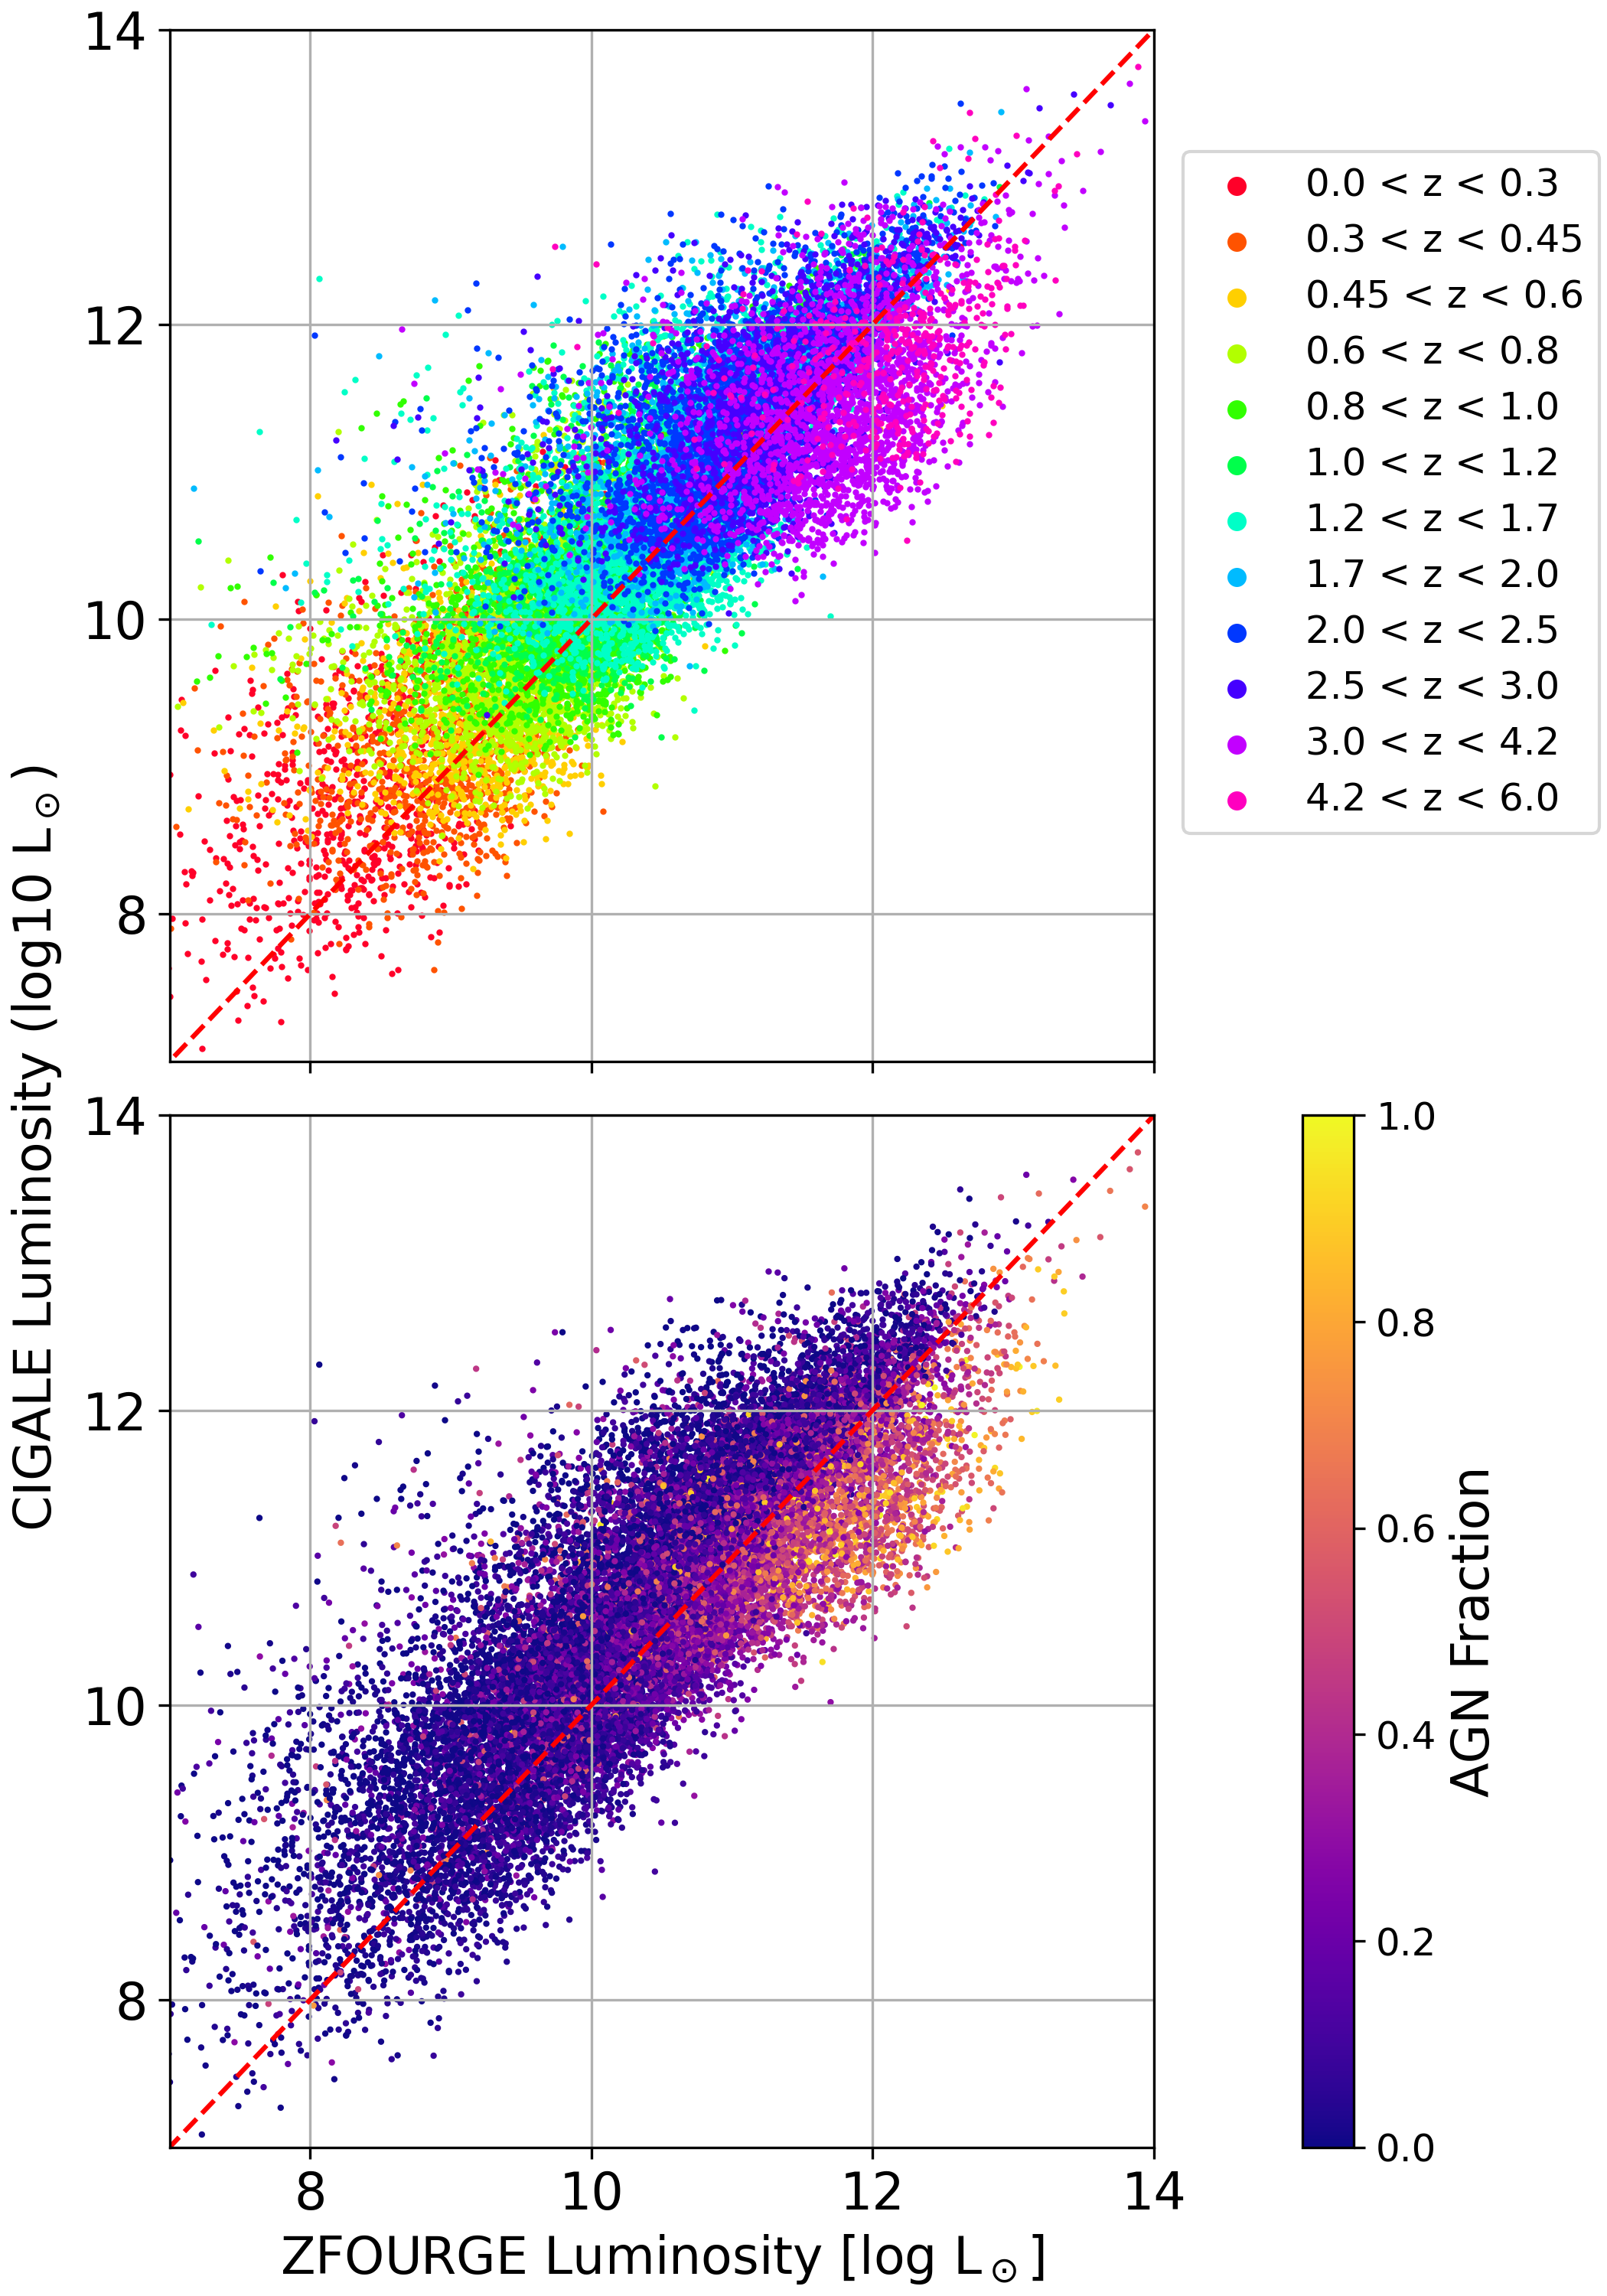
\includegraphics[width=0.48\textwidth]{Figures/LIR_vs_LIR.png}
    \caption{ZFOURGE bolometric 8-1000$\mu$m IR luminosity compared to CIGALE total luminosity. Top: Sources coloured by redshift bin. Bottom: sources coloured by AGN fraction ($\mathcal{F}_{AGN}$). AGN fraction increases with redshift. At $z \geq 3$, the average AGN fraction is greater than 30\%.}
    \label{Fig: LIR vs LIR}
\end{figure}

\subsection{Robustness Tests with Mock Analysis} \label{Sec: Mock_Analysis}
To ensure the reliability of the decomposition process, particularly for faint AGN, we performed a series of robustness tests using CIGALE's built-in mock analysis. These tests evaluate the software's ability to accurately decompose AGN and SF contributions across various redshifts and luminosities, specifically focusing on galaxies with low bolometric luminosities. By comparing the input and recovered AGN luminosities from the analysis, we confirmed that our parameter space and methodology are robust, particularly in detecting faint AGN. The mock analysis demonstrated that AGN luminosity was reliably constrained, with Pearson correlation coefficients (PCCs) ranging from 0.969 to 0.973 across all fields. Most sources lay within 0.5 dex of the 1-to-1 line, with mean residuals between $-0.02$ and $0.04$ dex, confirming the robustness of AGN luminosity recovery. These results indicate that our method effectively minimises bias against faint AGN, which are often difficult to detect in traditional analyses.

For a more comprehensive description of the SED decomposition methodology, see \cite{cowley_decoupled_2018}. Additionally, refer to the CIGALE software paper \citep{boquien_cigale_2019} for detailed information on its decomposition process and parameter optimisation techniques.

% \subsection{Bolometric IR Luminosity Derivation}
% \label{sec: Bolometric IR Luminosity}

% Understanding the total IR energy output of galaxies is essential for tracing both SF and AGN activity, particularly in dusty environments where much of the energy is re-emitted in the IR \citep{fu_decomposing_2010}. By estimating the bolometric IR luminosity, we can gain insights into the contribution of these processes across cosmic time. To this end, we integrate the best-fit SED of each source from 8-1000$\mu$m to estimate the bolometric IR luminosity, providing a robust measure of the total IR emission. Specifically, we use the averaged \cite{wuyts_fireworks_2008} template to fit the 24-160$\mu$m photometry, from which the total bolometric IR luminosity is derived. For a detailed description of this calculation, refer to section 6 of \cite{straatman_fourstar_2016}.

% Similarly, the CIGALE stellar and dust luminosity are combined to form the SF component. The CIGALE AGN luminosity forms the AGN component. These luminosities are subsequently used to construct the IR luminosity function of the ZFOURGE survey and CIGALE SF and AGN populations up to $z \approx 6$ (see section \ref{Sec: Luminosity Functions}). It is important to note that individual galaxies can contain both an AGN and SF component luminosity due to mixing. Figure \ref{Fig: SED Example} shows an example of a CIGALE SED and its decomposed components.

% The 24$\mu$m flux is usually a good proxy for the bolometric flux \citep{rodighiero_mid-_2010}. However, when the 24$\mu$m flux limit is used with the ZFOURGE bolometric luminosity, the limit varies with redshift, possibly due to spectral features shifting in and out of the template fitting process. Instead, we calculate the bolometric flux from the bolometric luminosity and take the 80\% completeness as the flux limit. We calculate the ZFOURGE bolometric flux limit to be $3.882\times10^{-18}$ $W/m^2$. The ZFOURGE star-forming and quiescent-dominated sources have very similar flux limits. \textcolor{red}{The CIGALE total and star-forming sources have a flux limit of $5.232\times10^{-18}$ $W/m^2$. The CIGALE AGN flux also varies with redshift, so we calculate the 80\% % completeness for each redshift bin. Additionally, luminosity completeness limits for ZFOURGE and CIGALE are calculated for each redshift bin. These limits represent the minimum luminosity a galaxy must have to be detectable throughout the entire redshift bin.}